%!TEX root=../protocol.tex	% Optional

\section{Einf{\"u}hrung}

Diese {\"U}bung zeigt die Anwendung von komponentenbasierter Programmierung mittels Webframeworks.

\subsection{Ziele}

Das Ziel dieser {\"U}bung ist die automatisierte Persistierung und Verwendung von Objekten eines vorgegebenen Dom{\"a}nenmodells mittels eines Frameworks. Dabei sollen die CRUD-Operationen der verwendeten API zur Anwendung kommen.

Die Persistierung soll mittels der Java Persistence API (JPA) realisiert werden.

\subsection{Voraussetzungen}

\begin{itemize}
    \item Grundlagen zu Java und das Anwenden neuer Application Programming Interfaces (APIs)
    \item Verst{\"a}ndnis {\"u}ber relationale Datenbanken und dessen Anbindung mittels h{\"o}herer Programmiersprachen (JDBC/ODBC)
    \item Verst{\"a}ndnis von UML und Build-Tools
\end{itemize}

\subsection{Aufgabenstellung}

Erstellen Sie von folgendem Modell Persistenzklassen und implementieren Sie diese mittels JPA:

\begin{figure}[h]
    \label{fig:uml}
    \centering
        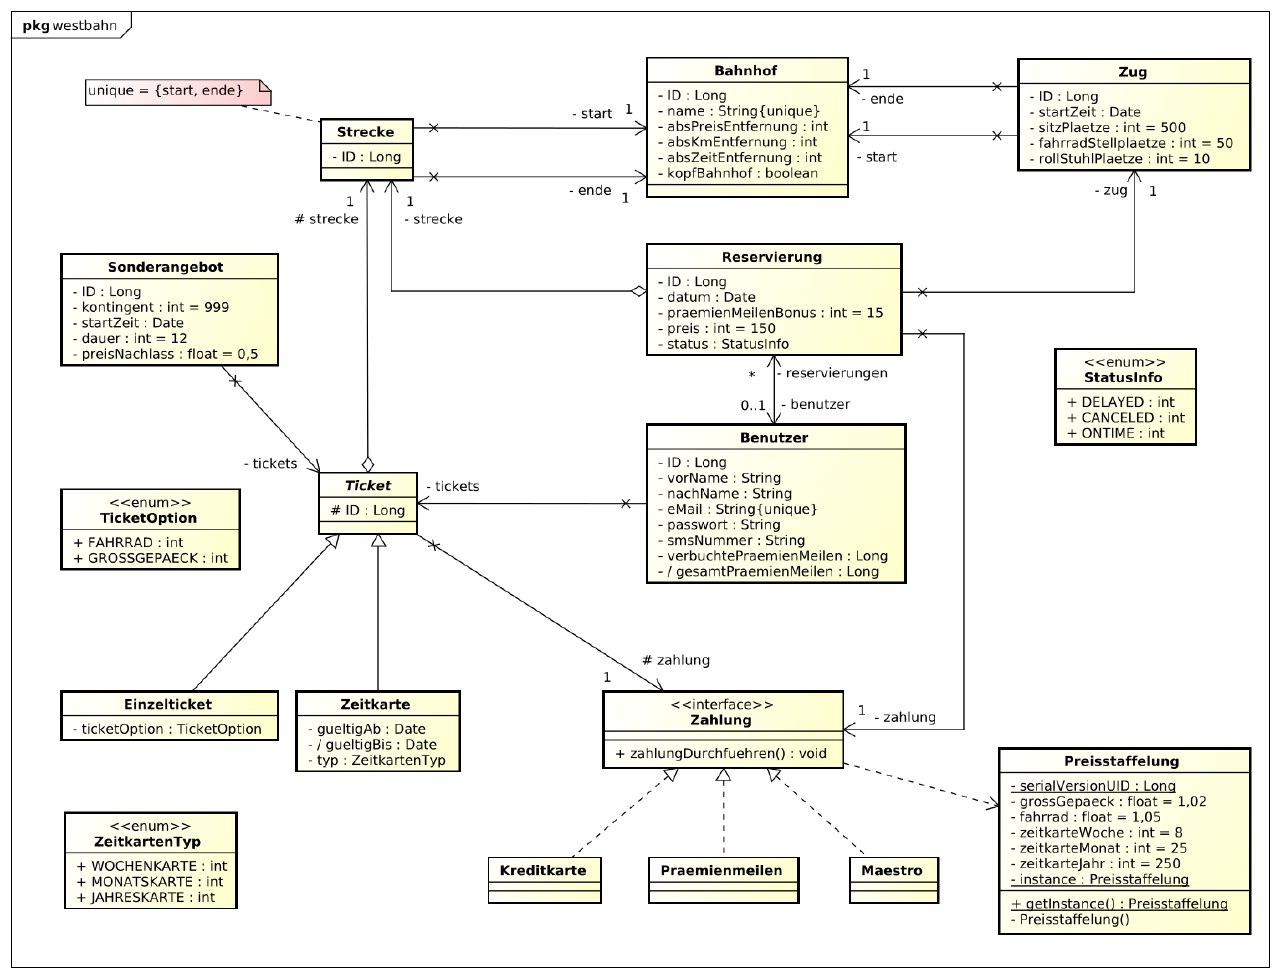
\includegraphics[width=\textwidth]{images/westbahn}
    \caption{Die Westbahn Datenstruktur (UML)}
\end{figure}

\paragraph{Suche}
Die Suche nach Z{\"u}gen muss auf jeden Fall die Auswahl des Abfahrts- und Ankunftsortes (nur folgende Bahnh{\"o}fe sind m{\"o}glich: Wien Westbhf, Wien H{\"u}tteldorf, St. P{\"o}lten, Amstetten, Linz, Wels, Attnang-Puchheim, Salzburg) erm{\"o}glichen. Dies f{\"u}hrt zur Anzeige der m{\"o}glichen Abfahrten, die zur Vereinfachung an jedem Tag zur selben Zeit stattfinden. Des weiteren wird auch die Dauer der Fahrt angezeigt.

In dieser Liste kann nun eine gew{\"u}nschte Abfahrtszeit ausgew{\"a}hlt werden. Die Auswahl der Zeit f{\"u}hrt zu einer automatischen Weiterleitung zum Ticketshop.

Um sich die Auslastung der reservierten Sitzpl{\"a}tze anzusehen, muss bei dem Suchlisting noch das Datum ausgew{\"a}hlt werden. Dieses Service steht jedoch nur registrierten Benutzern zur Verf{\"u}gung.


\paragraph{Ticketshop}
Man kann Einzeltickets kaufen, Reservierungen f{\"u}r bestimmte Z{\"u}ge durchf{\"u}hren und Zeitkarten erwerben. Dabei sind folgende Angaben notwendig:

Einzeltickets: Strecke (Abfahrt/Ankunft), Anzahl der Tickets, Optionen (Fahrrad, Großgep{\"a}ck)
Reservierung: Strecke (Abfahrt/Ankunft), Art der Reservierung (Sitzplatz, Fahrrad, Rollstuhlstellplatz), Reisetag und Zug (Datum/Uhrzeit)
Zeitkarte: Strecke, Zeitraum (Wochen- und Monatskarte)

Um einen {\"U}berblick zu erhalten, kann der Warenkorb beliebig bef{\"u}llt und jederzeit angezeigt werden. Es sind keine {\"a}nderungen erlaubt, jedoch k{\"o}nnen einzelne Posten wieder gel{\"o}scht werden.

Die Funktion „Zur Kassa gehen“ soll die Bezahlung und den Ausdruck der Tickets sowie die Zusendung per eMail/SMS erm{\"o}glichen. Dabei ist f{\"u}r die Bezahlung nur ein Schein-Service zu verwenden um zum Beispiel eine Kreditkarten- bzw. Maestrotransaktion zu simulieren.


\paragraph{Pr{\"a}mienmeilen}
Benutzer k{\"o}nnen sich am System registrieren um get{\"a}tigte K{\"a}ufe und Reservierungen einzusehen. Diese f{\"u}hren n{\"a}mlich zu Pr{\"a}mienmeilen, die weitere Verg{\"u}nstigungen erm{\"o}glichen. Um diese beim n{\"a}chsten Einkauf n{\"u}tzen zu k{\"o}nnen, muss sich der Benutzer einloggen und wird beim „Zur Kassa gehen“ gefragt, ob er die Pr{\"a}mienmeilen f{\"u}r diesen Kauf einl{\"o}sen m{\"o}chte.


Instant Notification System der Warteliste
Der Kunde soll {\"u}ber {\"a}nderungen bez{\"u}glich seiner Reservierung (Versp{\"a}tung bzw. Stornierung) mittels ausgesuchtem Service (eMail bzw. SMS) benachrichtigt werden. Bei ausgelasteten Z{\"u}gen soll auch die M{\"o}glichkeit einer Anfrage an reservierte Pl{\"a}tze m{\"o}glich sein. Dabei kann ein Zuggast um einen Platz ansuchen, bei entsprechender {\"a}nderung einer schon get{\"a}tigten Reservierung wird der ansuchende Kunde informiert und es wird automatisch seine Reservierung angenommen.


\paragraph{Sonderangebote}
F{\"u}r festzulegende Fahrtstrecken soll es erm{\"o}glicht werden, dass ein fixes Kontingent von Tickets (z.b.: 999) zu einem verbilligten Preis (z.b.: 50% Reduktion) angeboten wird. Diese Angebote haben neben dem Kontingent auch eine zeitliche Beschr{\"a}nkung. Der Start wird mit Datum und Uhrzeit festgelegt. Die Dauer wird in Stunden angegeben. Diese Angebote werden automatisch durch Ablauf der Dauer beendet.

\paragraph{Task 1 - Mapping}

Schreiben Sie f{\"u}r alle oben definierten Klassen und Relationen entsprechende Hibernate JPA Implementierungen (javax.persistence.*). Bis auf die Klasse Reservierung sollen daf{\"u}r die Annotationen verwendet werden. Die Klasse Reservierung soll mittels XML Mapping definiert werden.

\paragraph{Task 2 - Named Queries}

Schreiben Sie folgende NamedQueries (kein plain SQL und auch keine Inline-Queries) f{\"u}r das Dom{\"a}nenmodell aus Task1. Die Queries sollen die entsprechenden Parameter akzeptieren und die gew{\"u}nschten Typen zur{\"u}ckliefern:

\begin{enumerate}
    \item Finde alle Reservierungen f{\"u}r einen bestimmten Benutzer, der durch die eMail-Adresse definiert wird.
    \item Liste alle Benutzer auf, die eine Monatskarte besitzen.
    \item Liste alle Tickets f{\"u}r eine bestimmte Strecke aus (durch Anfangs- und Endbahnhof definiert), wo keine Reservierungen durchgef{\"u}hrt wurden.
\end{enumerate}

\paragraph{Task 3 - Validierung}

Alle Constraints der einzelnen Entit{\"a}ten sollen verifiziert werden. Hierf{\"u}r soll die Bean Validation API verwendet werden. Folgende Einschr{\"a}nkungen sollen {\"u}berpr{\"u}ft werden:

\begin{enumerate}
    \item Zug und Strecke k{\"o}nnen nicht denselben Start- und Endbahnhof besitzen.
    \item Die eMail des Benutzers soll ein g{\"a}ngiges eMail-Pattern befolgen.
    \item Die Startzeit eines Sonderangebotes kann nicht in der Vergangenheit liegen.
    \item Der Name eines Bahnhofs darf nicht k{\"u}rzer als zwei und nicht l{\"a}nger als 150 Zeichen sein. Sonderzeichen sind bis auf den Bindestrich zu unterbinden.
\end{enumerate}

\subsection{Bewertung}

\begin{itemize}
    \item Gruppengr{\"o}sse: 1 Person
    \item Anforderungen "{\"u}berwiegend erf{\"u}llt"
    \begin{itemize}
        \item Dokumentation und Beschreibung der angewendeten Schnittstelle
        \item Task 1
        \item Task 2
    \end{itemize}
    \item Anforderungen "zur G{\"a}nze erf{\"u}llt"
    \begin{itemize}
        \item Task 3
        \item Ausreichende Testobjekte zur Validierung der Persistierung
        \item {\"U}berpr{\"u}fung der funktionalen Anforderungen mittels Regressionstests
    \end{itemize}
\end{itemize}

\subsection{Quellen}

''The Java EE Tutorial - Persistence''; Oracle; online: https://docs.oracle.com/javaee/7/tutorial/partpersist.htm\#BNBPY

''HTML5 - A vocabulary and associated APIs for HTML and XHTML''; W3C; 17.12.2012; online: https://www.w3.org/TR/2012/CR-html5-20121217/forms.html\#valid-e-mail-address

''Hibernate ORM Documentation''; JBoss; online: http://hibernate.org/orm/documentation/5.2/l

''Hibernate ORM 5.2.13 Final User Guide''; JBoss; 25.01.2018; online: https://docs.jboss.org/hibernate/orm/5.2/userguide/html\_single/Hibernate\_User\_Guide.html
\clearpage
